\documentclass{beamer}
\usetheme[language=italian,
		  bullet=triangle,
		  color=blue,
		  titleline=true,
		  notshowauthor=true,
		  notshowtitle=true
         ]{TorinoTh}
\setbeamertemplate{caption}[numbered] % per avere fig. numerate nelle caption
\makeatletter
\renewcommand{\fnum@figure}{Fig. \thefigure} %per avere fig. invece che figura
\makeatother
\usepackage[beamer,customcolors]{hf-tikz}
\usepackage{graphicx}
\usepackage[font={footnotesize}]{caption}
\usepackage{wrapfig}

\hfsetfillcolor{alerted text.fg!10}
\hfsetbordercolor{alerted text.fg}

\begin{center}
\small Alma Mater Studiorum - Università di Bologna
\end{center}
\begin{center}
\small Scuola di Scienze - Corso di Laurea in Informatica
\end{center}

\author{Simone Preite}
\rel{Renzo Davoli}
\title{VSNLib: un'interfaccia unica di configurazione per stack virtuali tramite pacchetti netlink}
\ateneo{Università di Bologna}

%\date{Sessione II\\
%Anno Accademico 2016/2017\\ \\
%11 ottobre 2017} lo voglio fare uguale al frontespizio della tesi TODO

\date{20 dicembre 2017}

\begin{document}

\titlepageframe % Specific command


\begin{frame}[fragile]{Intro}
Il lavoro di tesi riguarda lo sviluppo di una libreria utile per facilitare la configurazione degli stack di rete virtuali  agli sviluppatori che intendono farne uso.
\end{frame}

\begin{frame}[fragile]{IPv6 vs IPv4}

\begin{itemize}
    \item IPv4 \`e insufficiente per fronteggiare la necessit\`a di nuovi indirizzi;
    \item Nodi sulla rete in continua ascesa, necessitano di nuovi indirizzi;
    \item IPv6: soluzione proposta gi\`a da diversi anni ma non ancora di largo utilizzo.
\end{itemize}
\end{frame}


\begin{frame}[fragile]{IoT}

\begin{columns}[T]
\begin{column}{.30\textwidth}
\newline
\begin{itemize}
    \item Connessione dispositivi comuni alla rete\newline
		\item Aumento esponenziale dei nodi\newline

\end{itemize}

\end{column}%
\hfill%
\begin{column}{.50\textwidth}
    \begin{figure}[t!]
    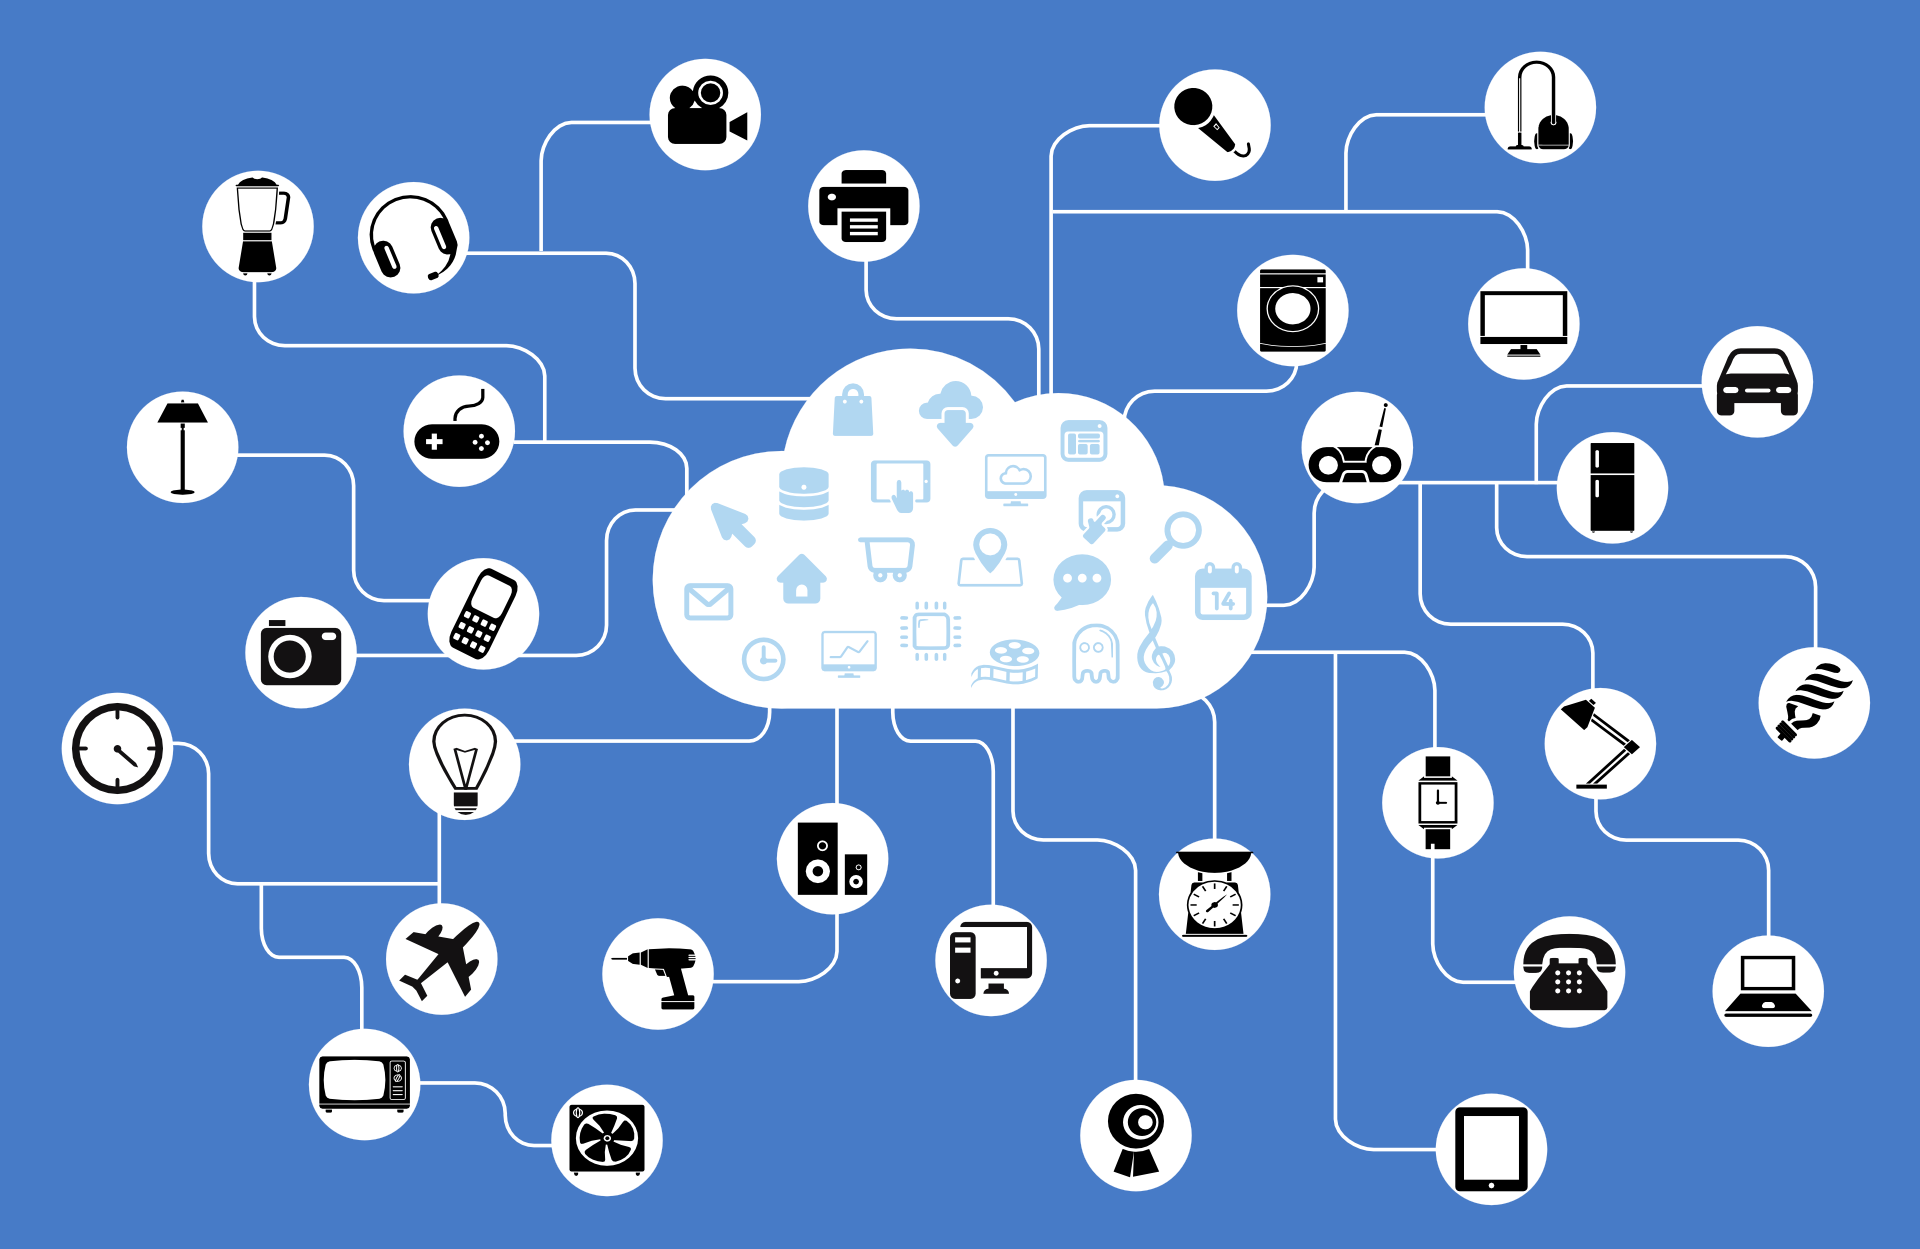
\includegraphics[scale=.08]{img/IoT.png}
    \caption{Internet of Things}
    \centering

\end{figure}
\end{column}%non mi piacciono le immagini
\end{columns}
\end{frame}

\begin{frame}[fragile]{IoTh}
	\begin{columns}[T]
	\begin{column}{.40\textwidth}
	    \begin{figure}[t!]
	    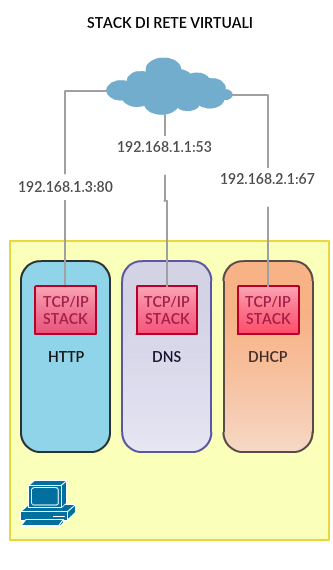
\includegraphics[scale=0.35]{img/new_stack.png}
	    \caption{Internet of Things}
	    \centering

	\end{figure}
	\end{column}%non mi piacciono le immagini
	\hfill%
	\begin{column}{.60\textwidth}
	\newline
	\begin{itemize}
	    \item Connessione di processi direttamente alla rete\newline
			\item Possibile grazie al gran numero di indirizzi IPv6\newline
			\item Paradigma simile alla telefonia mobile rispetto a quella fissa\newline
			\item \`E possibile trasferire processi da un capo all'altro del mondo senza problemi di indirizzamento e senza che il client si renda conto di nulla\newline
	\end{itemize}

	\end{column}%
	\end{columns}
\end{frame}

\begin{frame}[fragile]{Stack Virtuali}


		\begin{columns}[T]
		\begin{column}{.40\textwidth}
			\begin{minipage}[c][0.6\textheight]{\linewidth}
		 \begin{figure}[t!]
		    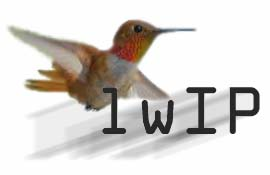
\includegraphics[scale=0.2]{img/lwip}
			    \caption{LWIP}
			\end{figure}
				\begin{figure}[t!]
		    
\includegraphics[scale=0.2]{img/picoTCP.png}
		    \caption{picoTCP}
			\end{figure}
\end{minipage}
		    \centering

		\end{column}
		\hfill%
		\begin{column}{.60\textwidth}
		\newline
		\begin{itemize}
		    \item PicoTCP\newline
				\item LightWeight IP (LWIP)\newline
				\item LightWeight IPv6 (LWIPv6)\newline

		\end{itemize}

		\end{column}%
		\end{columns}
		\vspace{1em}

		progetti di stack esistenti che permettono ai processi di comunicare tramite indirizzo personale

\end{frame}

\begin{frame}[fragile]{VSNLib}

Obiettivi di VSNLib:\newline
\begin{itemize}
    \item Windows (TightVNC)
    \item macOS (Vine Server/OSXvnc)
    \item GNU/Linux (x11vnc)

\end{itemize}

\begin{itemize}
    \item hostname
    \item modifica della risoluzione
    \item riduzione della parte di schermo da condividere
\end{itemize}
\end{frame}

\begin{frame}[fragile]{NETLINK}
	\begin{figure}[t!]
	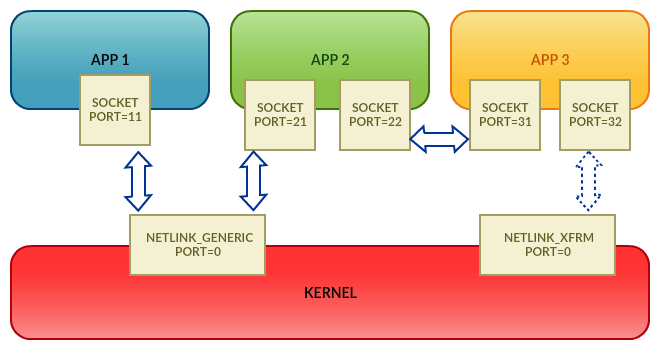
\includegraphics[scale=0.4]{img/netlink_comunication}
	\caption{netlink}
	\end{figure}
	\vspace{1em}
Netlink \`e un sistema di Inter Process Comminication (IPC), ovvero permette ai processi di scambiarsi messaggi.\\
Le porte utilizzate per la comunicazione sono create in funzione dei Process ID.\\
 %\begin{itemize}
    %\setlength\itemsep{2em}
    % \item Startup\newline
    % il client VNC viene eseguito in automatico all'avvio tramite creazione di desktop entry
%
  %   \item Indirizzo IP statico\newline
  %   viene abilitato modificando il file di configurazione del demone dhcpcd
  %   \item Blank screen\newline
  %   viene disabilitato agendo sul file di configurazione di LightDM, il display manager
 %\end{itemize}

 %%TODO magari dividere in due colonne e a dx mettere i listings...
\end{frame}

\begin{frame}[fragile]{FLUSSO}
 \begin{itemize}
   \setlength\itemsep{2em}
     \item Streaming audio e video
     \vspace{0.5em}
        \begin{itemize}
           \setlength\itemsep{0.5em}
        \item PulseAudio
        \end{itemize}
     \item File system read-only
     \vspace{0.5em}
        \begin{itemize}
        \setlength\itemsep{0.5em}
        \item Motivazioni
        \item Tabella delle partizioni
        \item UnionFS
        \item Abilitare temporaneamente la lettura-scrittura
        \end{itemize}

 \end{itemize}
\end{frame}

\begin{frame}[fragile]{CORE}

\begin{columns}[T]
    \begin{column}{.37\textwidth}
    \begin{itemize}
    \item Uso wireless\newline
    \small come estensione del Raspberry Pi Wireless Projector
    \item \normalsize Uso wired\newline
    \small in caso di disponibilità di soli proiettori tradizionali\\
    \end{itemize}

    \end{column}
    \begin{column}{.61\textwidth}
    \begin{figure}
        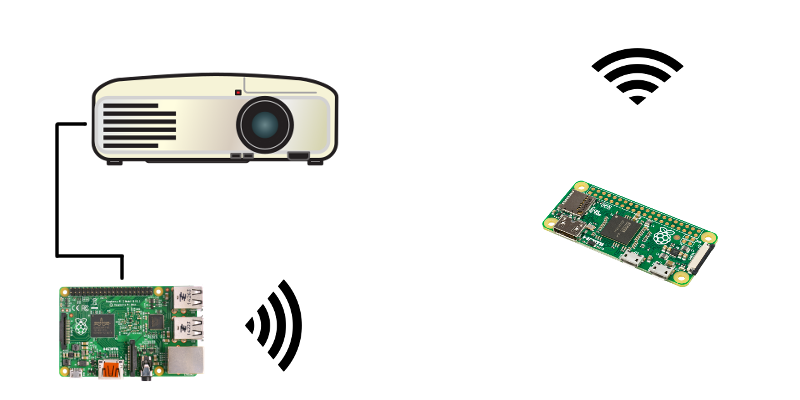
\includegraphics[scale=1.5]{img/setup-with-pizero.png}
        \caption{Uso wireless.}
    \end{figure}
    \end{column}
\end{columns}
\vspace{1em}

 La configurazione del sistema si basa sulla presenza di una directory predefinita che contiene le presentazioni e uno script che esegue all'avvio tramite file .desktop i programmi necessari per la presentazione: VNC (per uso wireless), Piremote, Evince.
\end{frame}

\begin{frame}[fragile]{MODULI}

\begin{columns}[T]
    \begin{column}{.48\textwidth}
    Disponibile a http://github.com/giulic3/piremote.

    \vspace{1em}
    Consente lo scorrimento delle pagine nella presentazione corrente, la navigazione all'interno della directory principale e l'apertura di nuove presentazioni.

    \end{column}
    \begin{column}{.48\textwidth}
    \begin{figure}
        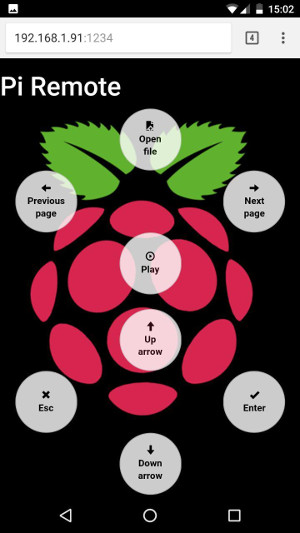
\includegraphics[scale=0.41]{img/main_page.jpg}
        \caption{Pagina di controllo di Piremote}
    \end{figure}
    \end{column}
\end{columns}
\end{frame}

\begin{frame}[fragile]{Conclusioni}
 \begin{itemize}
     \item Estensione del supporto server per dispositivi mobili (Android/iOS)
     \item Stabilità del canale nello streaming audio
     \item Tempi di avvio del Raspberry Pi Zero W
     \item Tempi di risposta in VNC on the GO
     \item Modalità di caricamento delle presentazioni
     \item Estensione delle possibilità di controllo tramite Piremote

 \end{itemize}
\end{frame}


\begin{frame}[fragile]{Sviluppi Futuri}
 \begin{itemize}
     \item Estensione del supporto server per dispositivi mobili (Android/iOS)
     \item Stabilità del canale nello streaming audio
     \item Tempi di avvio del Raspberry Pi Zero W
     \item Tempi di risposta in VNC on the GO
     \item Modalità di caricamento delle presentazioni
     \item Estensione delle possibilità di controllo tramite Piremote

 \end{itemize}
\end{frame}


\begin{frame}[c]

\begin{center}
\LARGE Grazie per l'attenzione\\
Domande?
\end{center}
\end{frame}

\begin{frame}[plain, noframenumbering]{Approfondimento: Limitazioni dei proiettori wireless}

Riguardano:\newline

\begin{itemize}

\item La tipologia di file trasmessi, con la mancanza di supporto video o risultati non soddisfacenti nella riproduzione
\item Le modalità di connessione, quando il servizio non è integrato in una rete esistente ma è richiesta la creazione di una rete ad hoc
\item Hardware aggiuntivo (es. adattatori USB) necessario per il funzionamento
\item I costi elevati, con differenze tra proiettori con WiFi built-in e proiettori tradizionali potenziati da adattatori wireless.

\end{itemize}
\end{frame}



\begin{frame}[plain, noframenumbering]{Approfondimento: File system e UnionFS}

\begin{itemize}
\item Tipo di file system che supporta union mount
\item È utilizzato per sovrapporre ad un sistema in sola lettura, un file system temporaneo memorizzato in RAM
\item Di conseguenza ogni scrittura avviene in RAM e verrà persa ad ogni riavvio, evitando potenziali scritture dannose su memoria SD.
\end{itemize}
\end{frame}

\begin{frame}[plain, noframenumbering]{Approfondimento: Piremote}

\begin{itemize}

\item Realizzato in Python, Javascript per il frontend
\item È basato su un modulo che consente il controllo completo di mouse e tastiera
\item Piremote può essere eseguito da riga di comando eventualmente specificando i parametri \textit{address}, \textit{port}, \textit{key}.

\end{itemize}

\end{frame}




\end{document}
